%\documentclass{article}
\documentclass[onecolumn]{IEEEconf}
%\usepackage{a4wide}
\usepackage{enumitem}
\usepackage[usenames, dvipsnames]{color}
\usepackage{graphicx}
\usepackage{subcaption}
\usepackage{ulem}
\renewcommand{\figurename}{Fig.}
\renewcommand*{\thetable}{\Roman{table}}

\title{Response to the Reviewers' Comments}
\begin{document}

\maketitle

The authors would like to thank the reviewers for the  comments and suggestions on the technical contents and presentation of our manuscript ``SmartPatch: A Self-Powered and Patchable Cumulative UV Irradiance Meter,'' submitted to IEEE Design and Test. This revised manuscript has been significantly improved thanks to the reviewers' invaluable advices. We have revised the manuscript faithfully following the reviewers' comments. We include the newly added or significantly modified parts in the revised version of the paper also in Response to Reviewers. We highlight the important technical content changes and set those parts in a red color in the revised paper. Detailed comments and corresponding corrections are listed below:\\

\setlength{\parindent}{0cm}
%%%%%%%%%%%%%%%%%%%%%%%%%%%%
\textbf{General Revision:}
We found that some unclear writing in Introduction could cause misleading in the technical contents while dealing with the reviewers' comments. We completely rewrite Introduction to deliver the technical contents more clearly.  We also corrected improper sentences, which were highlighted in red in the revised papers. Due to the page limit of IEEE Design and Test, we removed some less important sentences without hurting the technical contents at all.\\

\textbf{Reviewer 1:}
\setcounter{figure}{4} 
\begin{figure}[h]
\centering
	\begin{subfigure}{0.45\textwidth}
	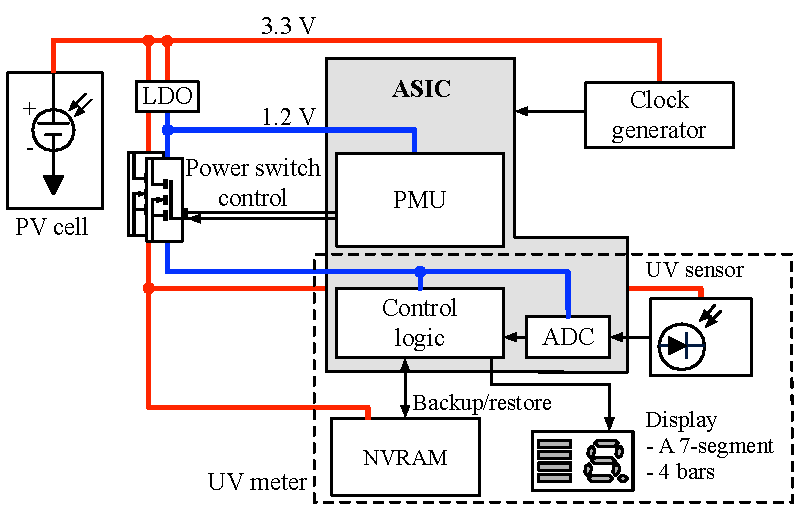
\includegraphics[width=1.0\hsize]{Figures/block_diagram.pdf}
	\caption{}
	\label{fig:block_diagram}
	\end{subfigure}
~
	\begin{subfigure}{0.45\textwidth}
	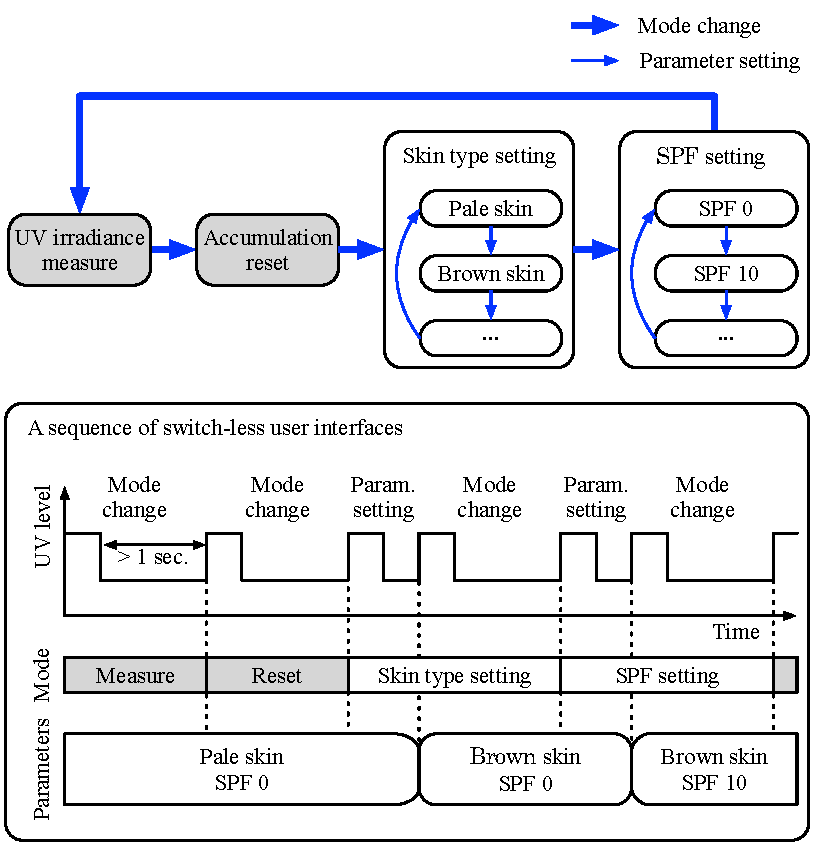
\includegraphics[width=1.0\hsize]{Figures/configuration.pdf}
	\caption{}
	\label{fig:configuration}
	\end{subfigure}
\caption{(a) A block diagram and \textcolor{red}{(b) mode change and parameter setting of SmartPatch.}}
\end{figure}
%%%%%%%%%%%%%%%%%%%%%%%%%%%%
\begin{description}
\item [C1: ] Is the number of modes a significant limitation of SmartPatch? It would also help to understand this if the amount MED varies with skin type is shown. If MED varies significantly between pale and very dark skin, and since SPF is multiplicative with maximum UV exposure time I would assume that the four modes does not cover the user space well. You could easily have more than two bins for skin type and way more sunscreen options (SPF 30+) that would significantly alter maximum UV exposure time.  
\item [R1: ] First of all, we modified the terms ``mode" to avoid confusion.``Mode" stands for the device \textit{operating modes}: measure, reset, skin type setting, and SPF setting" in the revised manuscript. We use ``parameter" setting that actually sets the skin type and SPF number in the revised manuscript. \\ \\
We do agree on the reviewer's comment on the user space. The previous implementation of had only one mode for the parameter setting, a combination of the user skin type and SPF number. As the reviewer pointed out, this certainly limits the user space due to a state explosion, not because of the hardware limit but because of time-consuming finger actions to cover a large user space. We looked down the importance of user convenience simply thinking this was for a demonstration purpose. However, we redesigned the control state machine of SmartPatch so that we separately set the skin type and SPF number in two different operating modes. \\ \\
We sincerely appreciate the reviewer to give us a chance not only for paper revision but also for design revision. We revised both Fig.~5 and related sentences on Page 4 as follows: \\ \\
\textit{\textcolor{red}{Fig.~\ref{fig:configuration} shows operation modes and user parameter setting for SmartPatch with the switch-less interface. The operating modes are measure, reset, skin type setting, and SPF setting. The mode changes one to the next in a round-robin manner when the UV sensor is blocked by a finger longer than a second. When the current mode is either skin type setting (or SPF setting), the current skin type (or the SPF number) changes to the next value if the UV sensor is blocked for a while, shorter than a half second. A longer blocking causes the mode change to the next while setting the parameter. The current design of SmartPatch accommodates up to 10 skin types and up to 10 SPF types for the demonstration purpose, but adding more skin and SPF types can easily be handled in a linear complexity of the parameter lookup table.}} \\
%
\item [C2: ] ``The existing UV meters under- or overestimates the accumulation of UV irradiance.'' I would assume that existing UV meters are accurate with respect to the part of the body it is monitoring. This should be corrected. In addition, is the shoulder the most appropriate place to measure the UV for these activities (e.g., chatting on a bench, walking outdoors, seated on a grass field)? For a person that is wearing a typical shirt, is the UV measurements in Fig. 9 given for their shoulder under their shirt? Or is the use-case more specific than that (e.g., tank tops or shirt-less)?
\item [R2: ] We agree on the reviewer's point. The existing UV meter is still accurate but can measure only limited body areas due to the design. So, it may under- or overestimate the UV irradiation of other body area of interest. We added one sentence on Page 5, the last paragraph of Section IV as follows:\\ \\
\textit{\textcolor{red}{The existing UV meter is still accurate but can measure only limited body areas due to the design. So, it may under- or overestimate the UV irradiation of other body area of interest.} This implies that watch type UV meters underestimate UV accumulation on the shoulder up to 16\%, which may cause 50\% more chances of erythema symptoms if UV exposure lasts until the watch type UV meters indicate the maximum exposure time is over~[2].}\\ \\
We also agree on our careless statement about the shoulder. For a more accurate presentation, we modify the the fourth paragraph of Section IV as follows:\\ \\
\textit{\textcolor{red}{To verify the functionalities and usefulness of SmartPatch, we compare the UV irradiance on various skin areas in the morning and afternoon as shown in Fig.~7. We measure the UV irradiation on the wrists, chests, shoulders, and from the ground as a reference.
In general, we usually get burned by the Sun when enjoying leisure on the beach. In particular, when walking on a beach, sitting on a bench or playing football, the most severe sunburn occurs on the shoulders if the person wears a sleeveless shirt or topless, for example. Therefore, we choose the shoulder as the skin area of interest in the experiment.}}
%
\item [C3: ] NVRAM should be defined at its first use.
\item [R3: ] We defined NVRAM (the non-volatile RAM) in the third row of the third paragraph in Section III-A as following:

\textit{DPM is no longer available if the solar irradiance becomes too low, and SmartPatch should be completely shut down. The power management unit (PMU) detects power interruption and allows the \textcolor{red}{nonvolatile RAM (NVRAM)} to store the necessary context[10].}\\
~\\

\item [C4:] The English and phrasing should be carefully reviewed. For example, it was difficult to parse ``We measure the UV irradiance on the wrists, chests� as a reference with several UV irradiance meters including SmartPatch (Fig. 2.).'' 

\item [R4: ] We apologize the grammar error in listing items. We revised the sentence as follows: \\ \\
\textit{\textcolor{red}{We measure the UV irradiation on the wrists, chests, shoulders, and the ground as a reference.} The skin area of interest in the experiment is the shoulder, and SmartPatch is attached to the shoulder skin.}\\
~\\

\item [C5:] Also, ``In cooperation with a sunscreen with a specific SPF and skin type, which are user programmable'' seems to imply that users can program their sunscreen's SPF and change their skin type and cooperation would imply that sunscreen can make their own actions. I believe it should be more along the lines of: SmartPatch can aid the user in when to reapply sunscreen based on the user's skin type and sunscreen SPF.

\item [R5: ] We apologize a mistake to make the sentence not properly read. We modify the sentence as follows:
\textit{\begin{itemize}
%\item Covering both the UVA and UVB spectrum,
\item Having a small form factor and possibly disposable,
\item \textcolor{red}{Allowing user parameter setting such as skin type and SPF number if sunscreen is applied,}
\item Calculating the maximum UV exposure time based on the UV irradiance and skin type,
\item A patchable design to measure the actual cumulative UV irradiance on the exact skin area of interest,
\item Self-powered by a PV cell with the minimum possible size, and
\item No use of a power converter nor significant energy storage.
\end{itemize}}

At the beginning of this research, we were going to attempt to notify when to reapply sunscreen. However, after research on sunscreen, it turns out that such notification is hard to achieve. Sunscreen fades away primarily due to friction (rubbing skin), wind and moisture (water and sweat.) So, it is virtually impossible to detect the remaining sunscreen on skin. Cosmetics companies and doctors simply recommend to reapply sunscreen after coming out from water, having a lot of sweat and also after every two hours, for instance. All sunscreens (and also UV irradiation meters) assume sunscreen is properly applied at all times.

\end{description}

\pagebreak


%%%%%%%%%%%%%%%%%%%%%%%%%%%%
\textbf{Reviewer 2:}
%%%%%%%%%%%%%%%%%%%%%%%%%%%%
\begin{description}
\item [C1: ] In abstract, you should address the motivation, your approach, and experimental results.

\item [R1: ] As the reviewer suggested, we update abstract as:

\textcolor{red}{Ultraviolet (UV) irradiance affects human bodies both positively and negatively. We introduce SmartPatch, a self-powered, small-form-factor, light-weight, low-cost, and a patch-type UV meter, that provides a scientific measure of UV radiation and irradiation on a particular skin area. It is powered by a tiny PV (photovoltaic) cell without a battery and a power converter and performs UI (user interface) without a physical switch.}\\
~\\

\item [C2: ] In Introduction, you can state your approach and the comparisons between your approach and the existing state-of-the-art approach.
\item [R2: ] As the reviewer suggested, we totally revise Introduction (Section I) to state our approach: 1) what normal people usually do to avoid excessive UV irradiance, 2) why we need more scientific information to consider individual's characteristics and 3) brief introduction to SmartPatch. In addition, we revise the backgrounds (Section II-B) to compare our implementation, SmartPatch, with the existing state-of-the-arts.\\

\uline{We modify the second paragraph in Section I to state 1) what normal people usually do to avoid excessive UV irradiance:}\\
%
\textcolor{red}{The intensity of UV irradiance is often quantified by the UV index (UVI). Region-based daily UVIs are commonly broadcasted through weather forecast channels. There are general guidelines to avoid skin damage classified with the UVI as shown in Fig.~1. For example, we are recommended to stay indoor when the UVI  is over 8.}\\

\uline{We modify the third and fourth paragraphs in Section I to state 2) why we need more scientific information considering individual's characteristics:}\\
%
\textcolor{red}{In order to safely perform outdoor activities without experiencing skin damage, we should be aware of  the maximum UV irradiation. UVI and UV exposure time are easy metrics to estimate UV irradiation for normal people when a medical-grade scientific measure is not accessible. Although we commonly estimate the UV irradiation by the UV exposure time, it cannot be a reasonable estimation of UV irradiation on a particular skin area because UV irradiation is determined by the time integral of the instantaneous UVI accounting the angle between the Sun, in addition to the individual factors such as skin color. Additional UV protection such as sunscreen lotion makes it even more difficult.} 

\textcolor{red}{It is crucial to directly measure the UV irradiance and irradiation on the target skin surface of interest, \textit{i.e.} a UV sensor must be directly mounted on the skin surface of interest with the same angle to the Sun. The UV meter continuously reads the UV sensor and integrates the value over time. Unfortunately, to the best of our knowledge, existing UV measuring tools for normal people (excluding a laboratory measurement setup) can hardly achieve this goal.}\\

\uline{We modify the fifth and sixth paragraphs in Section I to state 3) introduction to SmartPatch a solar powered patchable smart UV level meter:}\\
%
\textcolor{red}{In this article, we introduce SmartPatch, a solar-powered and patchable smart UV irradiation meter that informs both the current UV irradiance and irradiation. SmartPatch is designed to attach on the skin surface of interest, its UV measurement meets the above mentioned requirements such as the angle to the Sun, environmental change and body movement. Two key technologies are behind the proposed SmartPatch. The first is a storage-less and converter-less energy harvesting~[9] that does not require a battery nor a voltage converter for solar energy harvesting. The second is a switch-less user interface. These two technologies can significantly reduce both volumetric and gravimetric overheads as well as the manufacturing cost.}

\textcolor{red}{SmartPatch detects the correlation between the UV irradiance and solar irradiance. Natural operation keeps a high correlation between them. The correlation is broken if the UV sensor is intentionally blocked by a finger. SmartPatch detects such finger actions and utilizes them for UI (user interface) as if physical switches are pressed by the finger. A smartphone LED flashlight can do the same job. We design an app that  generates pre-defined light flashing patterns so that a single screen touch can replace multiple times of finger actions. These technologies make it possible to implement SmartPatch with simple integrated circuits in a single chip, and also make it possible for a tiny PV cell to directly supply power to the chip without a power converter and a battery. As a result, SmartPatch becomes extremely low-cost, low profile, small, and light.}

 \textcolor{red}{The main functions of SmartPatch include 1) displaying the current UVI, 2) displaying the remaining UV irradiation to avoid skin damage, and 3) mode change or parameter setting for the personalized skin type and the SPF (Sun protection factor) of the currently applied sunscreen lotion. We verified the functionalities and usefulness of SmartPatch performing various outdoor activities.}\\

\underline{We modify Section II-B to compare our implementation, SmartPatch, with the existing state-of-the-art:}\\
\textcolor{red}{There are various portable UV meters on the market as shown in Fig.~2(a). Most UV meters can only measure the instantaneous UVI though we emphasize UV irradiation measurement is meaningful. Some top-of-the-line UV meters (Fig.~2(b)) additionally inform UV irradiation. They are capable of notifying the maximum allowable UV exposure time based on the instantaneous UVI, skin type and SPF. In other words, the feature basically meets the requirement.  First, however, these devices typically include a battery~[5], [6]. The types of such class devices are often a wrist strap, a watch, a pendant, or a badge. So, second, such devices can only measure the UV irradiance of limited positions of the human body, which is unlikely vulnerable to sunburn.} 
%
As shown in Fig.~3, each skin surface area has a distinctly different amount of UV irradiance due to the different angle to the Sun. In addition, partial shading can continuously occur on each skin surface area by trees, buildings, other body parts, clothes, and so forth. For instance, people often experience skin damages on their shoulders while other skin areas (\textit{e.g.}, a wrist that has the UV strap) are manageable even if the whole body has been exposed to the Sun.

\textcolor{red}{Therefore, an accurate UV irradiation meter should position the UV sensor on the exact location of the target skin surface with the same perpendicular angle to the Sun. However, it is not practical to mount a separate UV sensor from the \textcolor{red}{UV meter main unit in Figs.~2(a) and~2(b)}. Therefore, a patchable design of a UV irradiance meter is only capable of measuring correct UVI. We easily figure out the most vulnerable skin area and attach the device onto it taking into account the environment, our outfit and activities. Recently, a patchable UV meter has been introduced by a cosmetic company as shown in Fig.~2(c)~[7]. It is powered by the user's smartphone via Near Field Communication (NFC.) However, the device should equipped with a large-size energy storage such as a supercapacitor and thus a power converter to continuously measure the UV irradiation after it has received energy from NFC.}\\
~\\

\item [C3: ] In Section II, authors state that "However they (devices) does not show the exact amount of accumulated UV irradiance." \\
1. Maybe the user does not care the exact amount of UV. \\
2. How do you know these devices cannot measure the exact amount? Do you have any literatures to support it?\\
3. In experiments, you also can compare your device with the existing devices to show how accuracy your device is.
\item [R3: ] 
1. We are sorry for the confused sentence. For clear understanding, we have significantly revise this section.\\
2. Typical UV meters cannot be attached on the skin area of interest, and they cannot measure the accurate amount of UV irradiance on that area.\\
3. To verify the functionalities and usefulness of SmartPatch, we compare the UV irradiance on various skin areas in different times of a day (in the morning and afternoon) as shown in Fig.~7. We measure the UV irradiation on the wrists, chests, shoulders, and from the ground as a reference. Please see fourth, fifth and sixth paragraphs in Section IV:\\

\textit{\textcolor{red}{To verify the functionalities and usefulness of SmartPatch, we compare the UV irradiance on various skin areas in the morning and afternoon as shown in Fig.~7. We measure the UV irradiation on the wrists, chests, shoulders, and from the ground as a reference.}
The skin area of interest in the experiment is the shoulder, and SmartPatch is attached to the shoulder skin. Other UV meters are carried or attached as designed. For instance, a watch type UV meter measures the UV irradiance on the wrist. The UV irradiance to the ground increases by the angle to the Sun that is the maximum at 1:36 pm (13:36) in the experiments.\\
%
Of course, the UV irradiance to the skin area is different by activities.
For example, playing soccer, working and walking outdoor cause high UV irradiance to the shoulder and chest as shown in Fig.7(a).
Unfortunately, the watch type UV meter on the wrist does not reflect the UV irradiance variation on the skin area of interest, i.e., shoulders, by the activities and the angle to the Sun.
However, it is impossible to put the watch type UV meter on the shoulder.
The UV irradiance to the shoulder is sometimes even larger than the UV irradiance to the ground when the shoulder has a perpendicular angle to the Sun.\\
%
We observe that existing UV meters under- or overestimate the accumulation of UV irradiance.
This implies that watch type UV meters underestimate UV accumulation on the shoulder up to 16\%, which may cause 50\% more chances of erythema symptoms if UV exposure lasts until the watch type UV meters indicate the maximum exposure time is over~[3].}\\
~\\

\item [C4: ] Also in Section II, the authors state that the reason why these devices are inaccurate is because every skin surface has a different perpendicular angle to the Sun. In your device, the reviewer wonders how you address this issue.
\item [R4: ] We implement a patchable UV level meter to directly attach on the skin area of interest. Two key technologies are behind the proposed SmartPatch to be a patchable device. The first is a storage-less and converter-less energy harvesting~[1] that does not require a battery nor a voltage converter for solar energy harvesting. The second is a switch-less user interface. These two technologies can significantly reduce both volumetric and gravimetric overheads as well as the manufacturing cost. To make the uniqueness of our work clear, we revised Introduction as follow:\\

\underline{We modify the fifth, sixth and seventh paragraphs in Section I in the manuscript as:}\\
\textcolor{red}{In this article, we introduce SmartPatch, a solar-powered and patchable smart UV irradiation meter that informs both the current UV irradiance and irradiation. SmartPatch is designed to attach on the skin surface of interest, its UV measurement meets the above mentioned requirements such as the angle to the Sun, environmental change and body movement. Two key technologies are behind the proposed SmartPatch. The first is a storage-less and converter-less energy harvesting~[9] that does not require a battery nor a voltage converter for solar energy harvesting. The second is a switch-less user interface. These two technologies can significantly reduce both volumetric and gravimetric overheads as well as the manufacturing cost.}

\textcolor{red}{SmartPatch detects the correlation between the UV irradiance and solar irradiance. Natural operation keeps a high correlation between them. The correlation is broken if the UV sensor is intentionally blocked by a finger. SmartPatch detects such finger actions and utilizes them for UI (user interface) as if physical switches are pressed by the finger. A smartphone LED flashlight can do the same job. We design an app that  generates pre-defined light flashing patterns so that a single screen touch can replace multiple times of finger actions. These technologies make it possible to implement SmartPatch with simple integrated circuits in a single chip, and also make it possible for a tiny PV cell to directly supply power to the chip without a power converter and a battery. As a result, SmartPatch becomes extremely low-cost, low profile, small, and light.}

 \textcolor{red}{The main functions of SmartPatch include 1) displaying the current UVI, 2) displaying the remaining UV irradiation to avoid skin damage, and 3) mode change or parameter setting for the personalized skin type and the SPF (Sun protection factor) of the currently applied sunscreen lotion. We verified the functionalities and usefulness of SmartPatch performing various outdoor activities.}\\
~\\

\item [C5: ] In experimental results, you should compare your results with the existing approaches and see what your improvements are in terms of power reduction and accuracy.
\item [R5: ] 
1. As mentioned in R3-3, we describe how our device is accurate compared with other existing approaches in Section IV in the manuscript:\\

\textit{We observe that existing UV meters under- or overestimate the accumulation of UV irradiance.
This implies that watch type UV meters underestimate UV accumulation on the shoulder up to 16\%, which may cause 50\% more chances of erythema symptoms if UV exposure lasts until the watch type UV meters indicate the maximum exposure time is over~[3].}\\

2. The power consumption of our product is low enough because the measured power consumption is lower than harvested power with the storage-less and converter-less energy harvesting technique. Please see the third paragraph in Section IV:\\

\textit{Finally, we measure the power consumption of the prototype including the ASIC. Table~III summarizes the power consumption of each component. The ASIC itself consumes 1.6 mW while the other peripherals consume 6.4 mW. In total, the prototype consumes 8 mW, which is low enough to use a small size PV cell (22 mm by 7 mm, 12.92 mW@$V_{MPP}$-3.4 V.) The final implementation will have a single chip ASIC including the NVRAM, an e-ink display and the optimal-size of PV cell on a flexible PCB. This is being lead by a company through technology transfer.}

\end{description}

\end{document}



